\section{Experimental Study}
\label{sec:exp}
In this section, we present our experimental findings on
deploying our GCMP detectors to large-scaled real trajectories.
All algorithms are were implemented in Java 1.7., and all the 
experiments are carried out on our in-house cluster: Dianwei. The cluster
includes 12 nodes, each of which is equipped with four quad-core 2.2GHz Intel processors,
32 GB memory and gigabit Ethernet. The cluster is installed with CentOS 5.5. 
operating system and Java 1.7.0 VM.

\textbf{Experiment Setup}: We use Yarn\footnote{http://hadoop.apache.org/docs/current/hadoop-yarn/hadoop-yarn-site/YARN.html}
to manage the cluster. One node is dedicated as Yarn's master node, and each other node reserves one core and 2 GB memory for
Yarn processes. We use Apache Spark~\cite{zaharia2012resilient} as the MapReduce framework. Spark takes
the remaining 11 nodes as the computing nodes.
To fully utilize the computing power of the cluster, 
we assign each node to run five executors, each executor takes three cores and 5 GB memory. We use "yarn-cluster" mode
for Spark which randomly picks one executor to act as the Application Master. Such a configuration allows us to run 162 tasks
at the same time. We use HDFS as our storage engine with replicator factor of 1.
The configurations of important parameters are summaries in the table below:



%\subsection{Implementation Issues}
%We use Apache Spark~\footnote{http://spark.apache.org/} as the experimental
%platform. Spark is one of the most popular MapReduce platform which
%uses in-memory cache to gain high speedup against Apache Hadoop~\cite{}. 
%Due to the direct support of MapReduce, our algorithm can be easily implemented in Spark. 
%In order to help reproduce our experiments, we further address some implementation issues.
%\subsubsection{Task Assignment}
%In spark, each task in reduce phase is an Apriori mining phase of 
%a star.
%Although our star partition method is theoretically balanced, 
%it is still necessary to assign equal number of tasks to each executors. 
%Spark naturally uses hashing to partition data into tasks, where such
%a partitioning does not care on the tasks size. In order to
%fully utilize the clusters, it is important to perform a weight-aware
%partition. In our implementation, we collect the number of edges
%in each star after map phase. Afterwards, we use a simple \emph{best-fit} strategy,
%where we assign stars in decreasing order with their sizes and each star
%is assigned to the currently least-loaded executor.  HERE WE MAY HAVE ANOTHER BOUND
%FROM LITERATURE, BUT I DIDN'T FIND YET. The injection of load balancing strategy
%between map and reduce phase can be naturally implemented in Spark, where the 
%map result can be cached and the reduce phase can be paused until when the
%partition strategy is ready.
%
%\subsubsection{Duplication Detection}
%It is notable that the patterns discovered from different tasks (stars) could
%be redundant due to containment relationship. For example, a pattern $\{a,b,c\}$
%can be discovered from the star $Sr_a$, while the pattern $\{b,c\}$ can be discovered
%from the star $Sr_b$. Though in most applications, such a duplicate pattern
%is permitted, we offer an option to eliminate these patterns. The strategy is 
%to broadcast each reducers output to every other reducers. This can be
%efficiently done via \emph{broadcast} variables~\footnote{http://spark.apache.org/docs/latest/programming-guide.html\#broadcast-variables} in Spark. Afterwards, each reduce can check 
%whether any resulted patterns are subsumed and thus filter those patterns.
%Theoretically, advanced techniques, such as Bloom Filters, can be applied to efficiently
%deal with the duplication detection. However, as the number of final patterns are
%normally quit small, we leave the exploration for those techniques to the future.
%
%\subsubsection{Handling Overlapping Clusters}
%When handling patterns such as \emph{flock} and \emph{group}, disk-based clustering
%on objects are applied. Such a clustering method may result one object belonging to
%multiple clusters. In such a case, just keeping the timestamps in the edge
%of connection graph is insufficient. Instead, we extend every timestemp $t$
%to a pair $\langle t,C \rangle$, where $C$ is the set of clusters objects
%belong to at time $t$. The only adaption we need to take the join during
%apriori phase. Given two timestamp set $T_1$ and $T_2$, the join result of
%$T_1$ and $T_2$ instead of being $\{\forall t | t\in T_1 \wedge t_\in T_2\}$,
%it changes to $\{\forall (t,C) | t\in T_1 \wedge t \in T_2 \wedge C = (T_1.C \cap T_2.C) \wedge C \neq \emptyset\}$.
%It is obvious to see the \emph{edge simplification} and \emph{candidate pruning} 
%still holds under this new setting.
%
%
%\subsection{Experimental Setup}
%We adapt one of the most popular MapReduce platform, Apache Spark, 
%to conduct experiments on mining GCMPs. 
%Our experiments run on a 9-node cluster, with Apache Yarn as
%the cluster manager. We use 1 node for Yarn resource manager, 
%and use the remaining 8 nodes as executors. Each node in the cluster
%is uniformly equipped with a 2.2GHz quad-core CPU with 32 GB memory. 
%Inter-node communication is carried by 
%the 1Gbps Ethernet.  Some critical configuration of Spark is 
%as follows:
\begin{table} [h]
\centering
\begin{tabular}{|l|c|}
\hline 
Parameter & Value  \\ 
\hline 
Java Version & 1.7.0 \\ 
\hline 
spark.driver.memory & 2GB \\ 
\hline 
spark.executor.cores & 3  \\ 
\hline 
spark.executor.instances & 54 \\ 
\hline 
spark.executor.memory & 5GB \\ 
\hline 
spark.master & yarn-cluster \\
\hline 
spark.serializer & KryoSerializer \\ 
\hline 
\end{tabular} 
\end{table}

\textbf{Datasets}: We prepare three real datasets for study. The details of the datasets are as follows:
\begin{itemize}
\item{Geolife}~\footnote{http://research.microsoft.com/en-us/projects/geolife/}: this dataset collects 
18,670 trajectories for passengers in Beijing over three years. The data are collected
per around 5 seconds. Each data point records a trajectory ID and the latitude/longitude information.
\item{Shopping}~\footnote{http://www.irc.atr.jp/crest2010\_HRI/ATC\_dataset/}: this dataset contains
 visitors trajectories in ATC shopping center in Osaka. The samples are taken per
 around 0.5 seconds. There are in total 13,183 trajectories. Each data point is a 
 trajectory ID with in-door coordinates.
\item{Taxi}: this dataset records 15,054 Singapore taxi trajectories over one month span. The sample 
rate is around 30 seconds. Each data point is the taxi plate with latitude/longitude.
\end{itemize}

\textbf{Preprocessing}: We replace timestamps with a global sequence for each dataset. The sequence number
$0$ is the earliest timestamp among all trajectories in a dataset. We use the sampling rate of 
each dataset as the tick of the sequence number and every data point is mapped to the nearest ticks. If
several points mapped to the same tick, they are merged by averaging the location coordinates.
For missing data within small intervals (i.e., sequence difference less than 10), 
we use linear interpolation to fill them. 
We then use DBSCAN ($\epsilon=5, minPt=10$ for GeoLife and Shopping, $\epsilon=20, minPt=10$ for Taxi)
as the clustering algorithm for preprocessing.  
Note that both our TRPM and SPARSE algorithms treat the preprocessing as a black box and other
spatial clustering methods are also applicable. The clustered snapshots are stored in HDFS in $\langle t, S_t \rangle$ pair, where
$t$ is the timestamp, $S_t$ contains the clusters at snapshot $t$. 
After preprocessing, the summary of statistics are presented as in Table~\ref{exp:dataset}. 
%But they are affected by the number of clusters at each snapshot. We measure the 
%effect of different clustering parameters later. 

\begin{table} [h]
\center
\small
\begin{tabular}{|l|l|l|l|}
\hline
 \textbf{Attributes}& \textbf{Geolife} & \textbf{ACTShopping} & \textbf{SingTaxi} \\ 
\hline 
\# objects & 18,670 & 13,183 & 15,054\\ 
\hline
\# average ts & 2,924 & 3,114 & 19,667 \\ 
\hline
\# data points & 54,594,696 & 41,052,242 & 296,075,837\\ 
\hline
\# snapshots & 10,699 & 16,931 & 44,364\\ 
\hline
\# clusters & 206,704 & 211,403 & 536,804\\
\hline
avg. cluster size & 223 & 171 & 484\\
\hline
\# of patterns & 441 & 369 & 585 \\
\hline
\end{tabular}
\caption{Statistics of data set}
\label{exp:dataset}
\end{table}

\textbf{Parameters}: We study the performance of 
the GCMP detectors under various conditions. The variables
to be tested and their value ranges are listed in Table~\ref{tbl:parameters}. 
The default values are highlighted in bold.
\begin{table}[h]
\small
\begin{tabular}{c|l|l}
\hline 
\textbf{Variables} & \textbf{Meaning} & \textbf{Values} \\ 
\hline 
M & min size of object set &  5, 10,  \textbf{15}, 20, 25 \\ 
\hline 
K & min duration & 120, 150, \textbf{180}, 210, 240 \\ 
\hline 
L & min local duration & 10, 20, \textbf{30}, 40,50 \\ 
\hline 
G & max gap & 10, 15, \textbf{20}, 25, 30 \\ 
\hline
N & number of executors & 1, 14, 24, 34, 44, \textbf{54}\\ 
\hline 
\end{tabular} 
\caption{Variables and their default values during experiments.}
\label{tbl:parameters}
\end{table}

\subsection{Effects of $G$ on GCMP}
\begin{figure*}[t]
\centering
    \begin{subfigure}[b]{0.3\textwidth}
        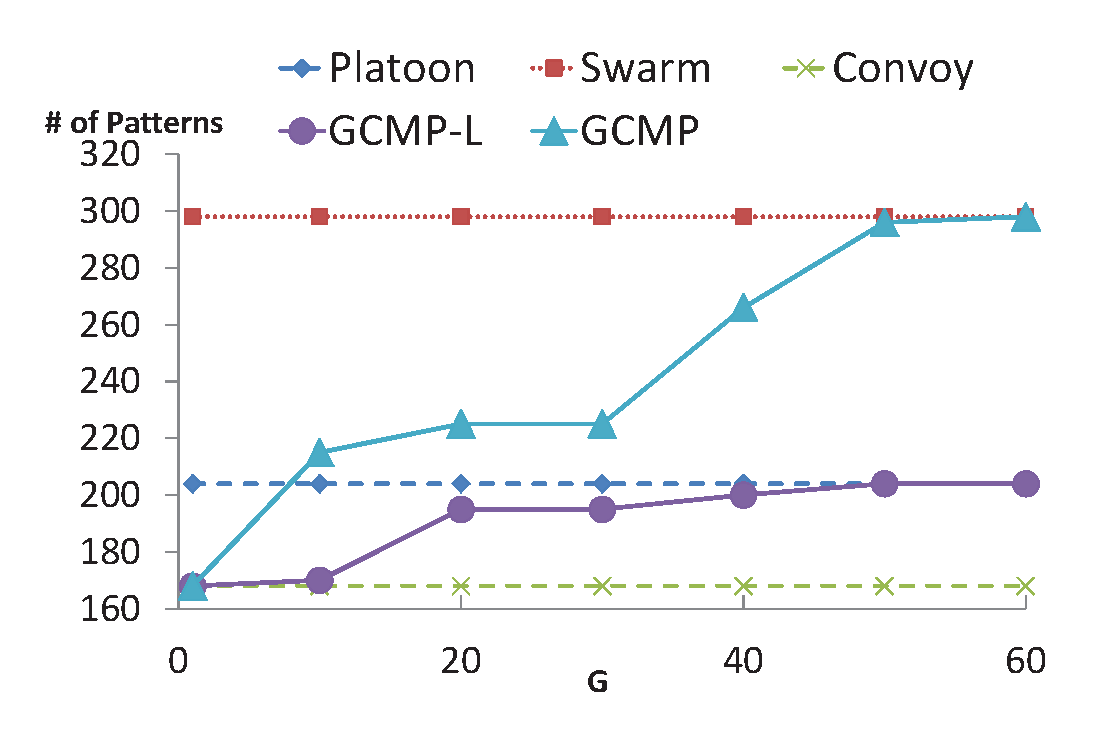
\includegraphics[width=\textwidth]{exp/effectiveness/effect_geolife.eps}
        \caption{Geolife}
    \end{subfigure}
    \begin{subfigure}[b]{0.33\textwidth}
        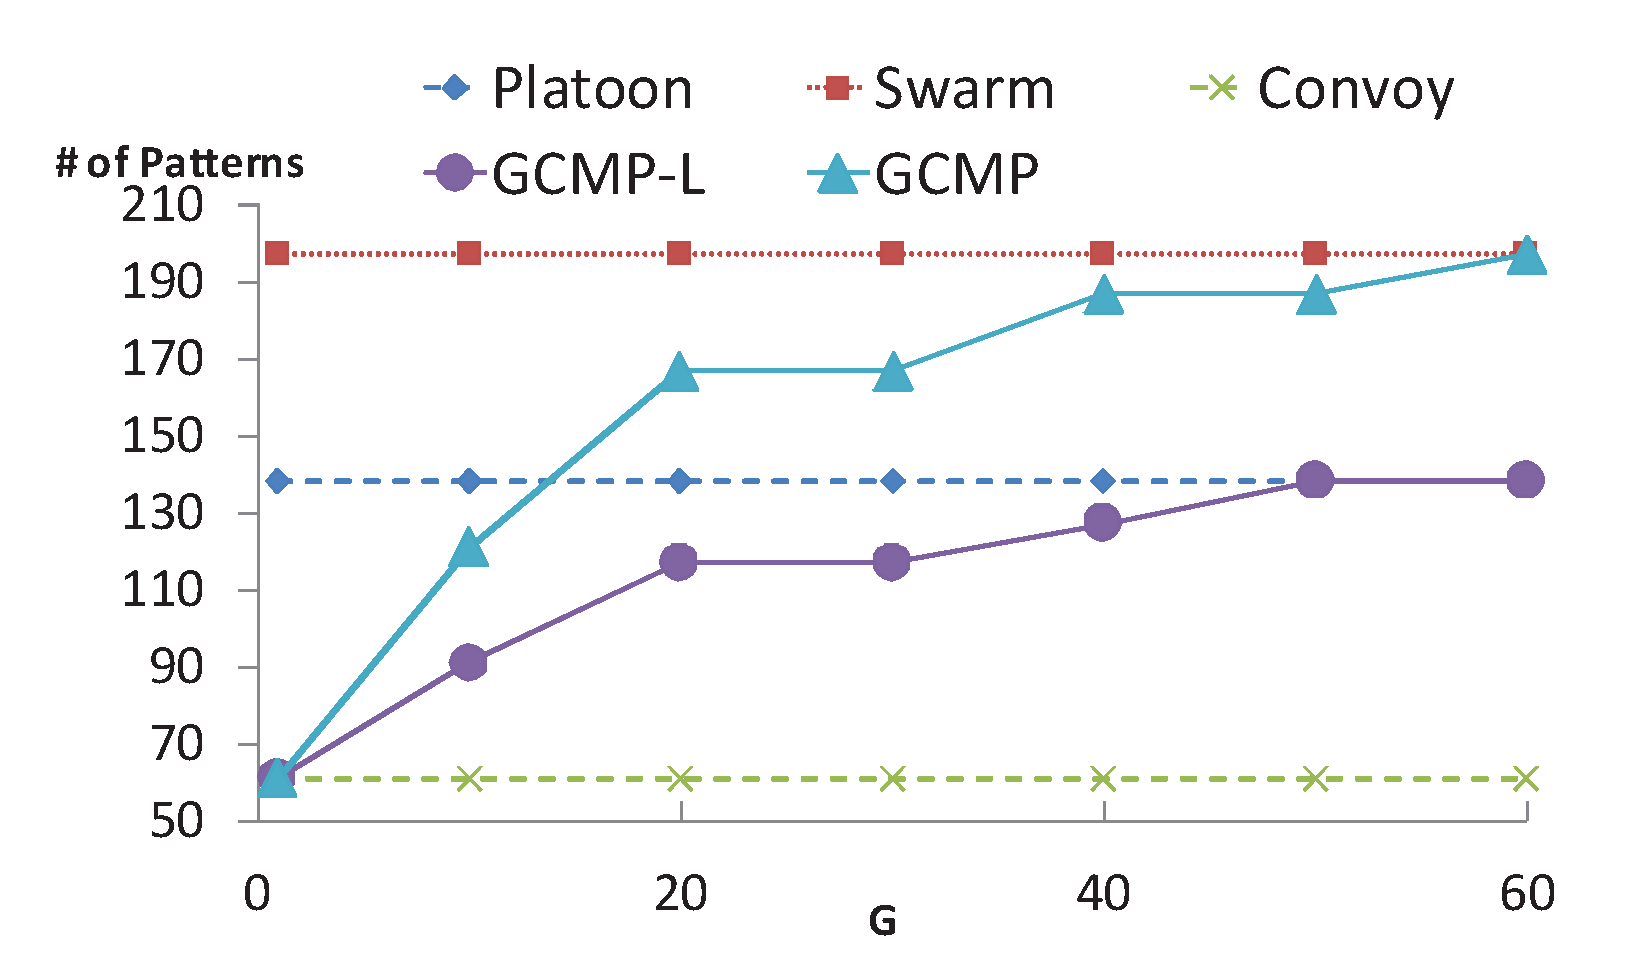
\includegraphics[width=\textwidth]{exp/effectiveness/effect_shopping.eps}
        \caption{ACTShopping}
    \end{subfigure}
    \begin{subfigure}[b]{0.3\textwidth}
        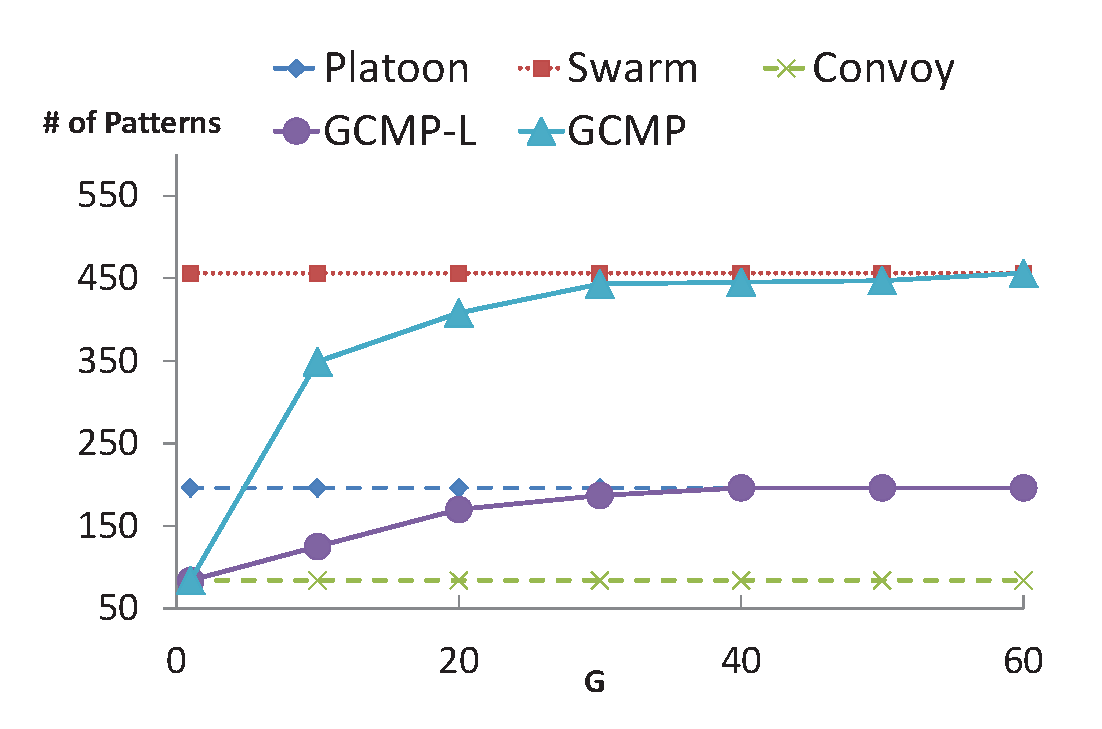
\includegraphics[width=\textwidth]{exp/effectiveness/effect_taxi.eps}
        \caption{SingTaxi}
    \end{subfigure}
\caption{Effectiveness of GCMP model on sampled datasets.}
\label{exp:effectiveness}
\end{figure*}
We first study the effects of introducing gap parameter $G$ on pattern discovery.
As shown in Figure~\ref{fig:related_work_scalability},
existing works are not able to handle large trajectories, 
we sample and cluster $1$ million trajectory points from the three real data.
We use two instances of GCMPs, GCMP-L where the $L$ value is default and GCMP where $L = 1$.  We measure the number
of patterns discvoered by different methods. The results are presented in Figure~\ref{exp:effectiveness}.

We can see from Figures~\ref{exp:effectiveness} that the number of patterns
discovered by GCMP is positively related to $G$. When $G =1$, the number
of patterns returned by GCMP and GCMP-L are identical to \emph{convoy}. As $G$ grows,
the number returned by GCMP-L converges to \emph{platoon}. For example, in (a), two
patterns converge when $G$ is $40$. Similarly in (b) and (c), two patterns converge
when $G$ is $50$. The reason is that when $G$ is large enough,
 all \emph{platoon}s are $G$-connected. Similar
 trend applies between GCMP and \emph{swarm}. As see from the figures, in (a), two
 patterns converge at $G=50$; while in (b) and (c) the two patterns converge
 at $G=60$ and $G=40$ respectively. We further
 note that, existing patterns has different granularity in temporal domain. As we seen
 from the three figures, the number of \emph{swarm} is greater than \emph{platoon} and
 \emph{convoy}. Despite none of the existing patterns are able to fine-grain control
 the temporal domain of patterns, GCMP can discover the patterns more precisely. 
 These results confirms the usefulness of GCMP in expressing other patterns.
  



\subsection{Performance Comparison}
%\textbf{Default Setting}: We now analyze the TRPM and SPARE algorithm under different
%parameter settings. Under the default parameter settings,
%the performance of TRPM and SPARE is shown as in the 
%following table:
%\begin{table}
%\small
%\begin{tabular}{|c|c|c|c|c|c|c|}
%\hline 
%Data Set& \multicolumn{2}{c|}{TRPM} & \multicolumn{2}{c|}{SPARE} & \# Patterns \\ 
%\hline 
% & Map-Shuffle & Reduce & Map-Shuffle & Reduce &  \\ 
%\hline 			
%Shopping &55 & 279 & 183 &414 &369\\ 
%\hline
%GeoLife &72 & 408 & 162 &585 &441  \\
%\hline
%Taxi &193 & 619 & 562 &3086 &585 \\
%\hline 
%\end{tabular} 
%\caption{Detail performance of TRPM and SPARE under default parameters.}
%\end{table}
%
%As can be seen from the above table, the number of patterns
%discovered by the default parameters are up to five hundreds.
%Thus, the parameter settings are reasonable. Besides, we 
%can see that TRPM suffers from shuffle and mining process. 
%This is because $\eta$ is set to be $309$ under default parameters.
%As a comparison, SPARE takes only in average
% 36\% of TRPM's shuffle time. 
To study the performance of TRMP and SPARE, we run both algorithms 
in all three datasets under different parameter settings. We report
their overall performance as in Figures~\ref{exp:performance_vary}.
In brief, both algorithms are able to handle the large-scaled real
datasets. However, we observe that TRMP's performance is very
dependent on the pattern parameters.
In cases when $G$ is large, TRMP takes near three hours (e.g., in Taxi dataset).
In contrast, SPARE performs quite stable. Another general observation
is that both algorithms run slower in the Taxi dataset as compared to in
other two datasets. This is because Taxi dataset contains
the most number of temporal data points, which is around 7 times of Shopping
dataset and 5 times of geolife dataset. We observe that, 
in almost all cases, SPARE outperforms TRMP and analyze the detail
of each scenario separately:

\textbf{Vary $M$}: Figures~\ref{exp:performance_vary} (a),(e),(i)
present the performance of TRPM and SPARE when $M$ changes under three datasets.
As the figures show, SPARE runs much faster than TRPM. We can see that SPARE
speeds up TRPM 2.7 times in Shopping data, 3.1 times in Geolife data and
7 times in Taxi data. Another observation is that, the running times
of both algorithms slightly decrease as $M$ grows. This is
because when $M$ becomes bigger, smaller clusters (stars) in 
the reduce phase of TRPM and SPARE can be directly pruned.

\textbf{Vary $K$}: Figure~\ref{exp:performance_vary} (b),(f),(j) 
presents the performance of TRPM and SPARE when $K$ changes under three datasets. 
There are two interesting findings in study the performance wrt. $K$. 
First, SPARE and TRPM takes different trends as $K$ increases. 
Whe $K$ increases, SPARE tends to have faster performances 
while TRPM's performances continuously slow down. For SPARE, the 
good performances result from more pruning powers brought
by $K$. When $K$ increases, many shorter time sequences in the reduce phase
are pruned. In contrast, $K$ does not bring much pruning power
during the reduce phase of TRPM. Even $K$ is very large, each reducers in TRPM
still has to sweep the entire partition to determine whether a pattern exists.
Moreover, $\eta$ in TRPM grows linearly with $K$. This indicates that
more data are shuffled and more snapshots are need to
be swept in each partition. This explains the low performance of TRPM as $K$
increases. Another interesting finding is that, when $K$ is small,
TRPM tends to outperform SPARE. This is because that when $K$ is small, shuffle
data of TRPM is comparable to SPARE. Meanwhile, small $K$ indicates small
size of partition in TRPM but low pruning power in SPARE. This explains the
superiority of TRPM. Note that, when $K$ is small, TRPM is at most 1.3 times
faster than SPARE and the absolute time is less than three minutes. 

\textbf{Vary $L$}:Figure~\ref{} presents the performance
of TRPM and SPARE when $L$ changes under three datasets.

\textbf{Vary $G$}:Figure~\ref{} presents the performance
of TRPM and SPARE when $G$ changes under three datasets.

%\subsubsection{Effects of clusters $\epsilon$, minPt}

\begin{figure*}[t]
\centering
    \begin{subfigure}[b]{0.23\textwidth}
        \includegraphics[width=\textwidth]{/exp/performance/shopping_vary_M.eps}
        \caption{Shopping Vary $M$}
    \end{subfigure}
    \begin{subfigure}[b]{0.23\textwidth}
        \includegraphics[width=\textwidth]{/exp/performance/shopping_vary_K.eps}
        \caption{Shopping Vary $K$}
    \end{subfigure}
    \begin{subfigure}[b]{0.23\textwidth}
        \includegraphics[width=\textwidth]{/exp/performance/shopping_vary_L.eps}
        \caption{Shopping Vary $L$}
    \end{subfigure}
       \begin{subfigure}[b]{0.23\textwidth}
        \includegraphics[width=\textwidth]{/exp/performance/shopping_vary_G.eps}
        \caption{Shopping Vary $G$}
    \end{subfigure}

	\begin{subfigure}[b]{0.23\textwidth}
        \includegraphics[width=\textwidth]{/exp/performance/geolife_vary_M.eps}
        \caption{Geolife Vary $M$}
    \end{subfigure}
    \begin{subfigure}[b]{0.23\textwidth}
        \includegraphics[width=\textwidth]{/exp/performance/geolife_vary_K.eps}
        \caption{Geolife Vary $K$}
    \end{subfigure}
    \begin{subfigure}[b]{0.23\textwidth}
        \includegraphics[width=\textwidth]{/exp/performance/geolife_vary_L.eps}
        \caption{Geolife Vary $L$}
    \end{subfigure}
       \begin{subfigure}[b]{0.23\textwidth}
        \includegraphics[width=\textwidth]{/exp/performance/geolife_vary_G.eps}
        \caption{Geolife Vary $G$}
    \end{subfigure}
    
    \begin{subfigure}[b]{0.23\textwidth}
        \includegraphics[width=\textwidth]{/exp/performance/taxi_vary_M.eps}
        \caption{Taxi Vary $M$}
    \end{subfigure}
    \begin{subfigure}[b]{0.23\textwidth}
        \includegraphics[width=\textwidth]{/exp/performance/taxi_vary_K.eps}
        \caption{Taxi Vary $K$}
    \end{subfigure}
    \begin{subfigure}[b]{0.23\textwidth}
        \includegraphics[width=\textwidth]{/exp/performance/taxi_vary_L.eps}
        \caption{Taxi Vary $L$}
    \end{subfigure}
       \begin{subfigure}[b]{0.23\textwidth}
        \includegraphics[width=\textwidth]{/exp/performance/taxi_vary_G.eps}
        \caption{Taxi Vary $G$}
    \end{subfigure}       
\caption{Performance of SPARE and TRPM on real datasets under different pattern parameters.}
\label{exp:performance_vary}
\end{figure*}


\subsubsection{Effects of pattern parameters $M,L,K,G$}

\subsection{SPARE Analysis}
\subsubsection{Load Balance}
\subsubsection{Scalability}



